\capitulo{3}{Conceptos teóricos}

En este capítulo se explican los conceptos teóricos indispensables para comprender la implementación del sistema.

\section{Blender y modelado 3D}

Blender es un programa de edición de gráficos que se emplea para diseñar y crear objetos 3D. El software se usa en videojuegos, animación, arquitectura o fabricación 3D.

El modelado 3D se refiere al desarrollo de modelos dentro un entorno 3D. Los objetos son formados mediante vértices, aristas y caras. A través de estas estructuras, los modelos pueden ser de simple o gran complejidad.

\begin{itemize}
\item Los vértices son como los puntos que marcan algo en el espacio.
\item Las aristas unen esos puntos.
\item Y las caras son las superficies que podemos ver del modelo.
\end{itemize}

La Figura~\ref{fig:blender_interface} muestra un cubo en un espacio 3D dentro de la interfaz de Blender.

% 3.1 Blender y modelado 3D
\begin{figure}[H]
    \centering
    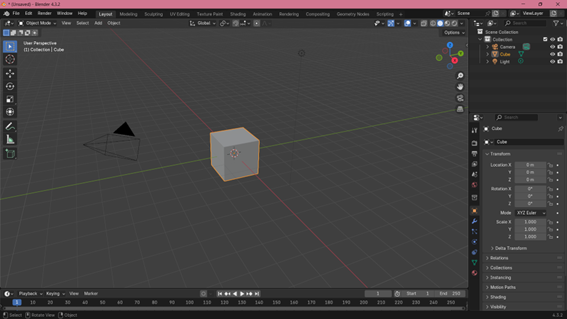
\includegraphics[width=0.9\textwidth]{diagramas/3.1blender_interface.png}
    \caption{Interfaz general de Blender durante una sesión de modelado.}
    \label{fig:blender_interface}
\end{figure}

Cuando estás modelando, el usuario hace cosas como:

\begin{itemize}
\item mover objetos,
\item añadir piezas,
\item cambiar vértices,
\item aplicar cambios (como rotar o escalar),
\item pasar de un modo de edición a otro,
\item usar modificadores,
\item o ajustar las coordenadas UV, que es para colocar las texturas sobre el modelo 3D.
\end{itemize}

Todo esto que haces va generando cambios dentro de la escena. Nuestro sistema justamente se aprovecha de esos cambios para ir recogiendo datos sobre cómo se está desarrollando el modelado.

\section{Addons}

Un \textit{addon} es como un pequeño extra que le puedes añadir a Blender para que haga más cosas, y se hace con código Python.

Gracias a esto, podemos crear herramientas a medida sin tener que tocar el programa principal de Blender.

Los \textit{addons} sirven para que Blender pueda tener, por ejemplo:

\begin{itemize}
\item herramientas para automatizar tareas,
\item sistemas de animación,
\item formas de exportar modelos,
\item herramientas para renderizar,
\item o sistemas para analizar datos.
\end{itemize}

Para este proyecto, hemos creado dos \textit{addons}:

\begin{itemize}
\item uno para capturar datos,
\item y otro para analizarlos y verlos de forma gráfica.
\end{itemize}

Aparte de los \textit{addons} que hemos hecho aquí, Blender ya viene con muchos otros que se usan mucho en el ámbito profesional. Aqui hay algunos ejemplos:

\begin{itemize}
\item Node Wrangler: te hace la vida más fácil cuando trabajas con materiales y nodos.
\item LoopTools: añade algunas herramientas más avanzadas para editar la geometría.
\item Rigify: te ayuda a crear esqueletos para animar de forma automática.
\item Archimesh: sirve para generar elementos de arquitectura de manera automática.
\end{itemize}

La Figura~\ref{fig:addons_menu} muestra el menú de \textit{addons} dentro de Blender.
% 3.2 Addons
\begin{figure}[H]
    \centering
    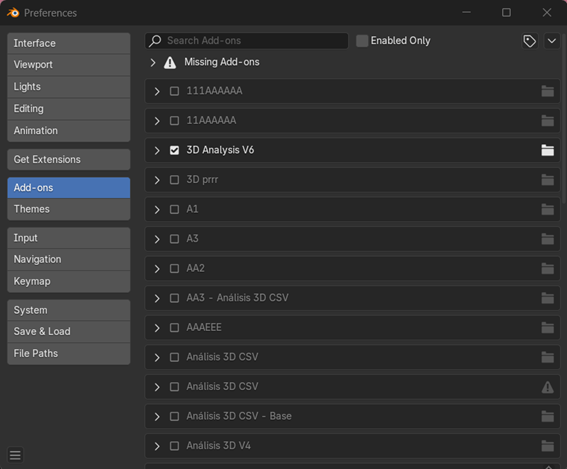
\includegraphics[width=0.75\textwidth]{diagramas/3.2addons_menu.png}
    \caption{Menú de \textit{addons} de Blender con extensiones instaladas.}
    \label{fig:addons_menu}
\end{figure}

Cada vez que haces algo en Blender, la escena cambia.

Blender tiene unos mecanismos internos, que se llaman \textit{handlers}, que detectan estos cambios de forma automática.

El sistema que hemos creado usa estos \textit{handlers} para registrar solo los cambios que realmente nos interesan.

Por ejemplo, cosas como:

\begin{itemize}
\item cuando creas objetos,
\item cuando borras partes de la geometría,
\item cuando cambias de modo (de edición, por ejemplo),
\item cuando modificas la geometría,
\item cuando mueves o rotas cosas en el espacio,
\item o cuando cambias las coordenadas UV (\textit{sistema utilizado para mapear texturas 2D sobre superficies 3D}).
\end{itemize}

Así es como funciona el proceso general para capturar estos datos:

\begin{enumerate}
\item Tú, como usuario, haces algo en Blender.
\item Blender actualiza lo que ves en la escena.
\item Nuestro sistema se da cuenta de que algo ha cambiado.
\item Se mira si ese cambio es importante para nosotros.
\item Si lo es, se guarda la información.
\item Después, podemos analizar y ver esos datos.
\end{enumerate}

La Figura~\ref{fig:flujo_eventos} muestra de forma resumida el flujo de eventos de detección y registro de datos.

%3.3
\begin{figure}[H]
    \hfill
    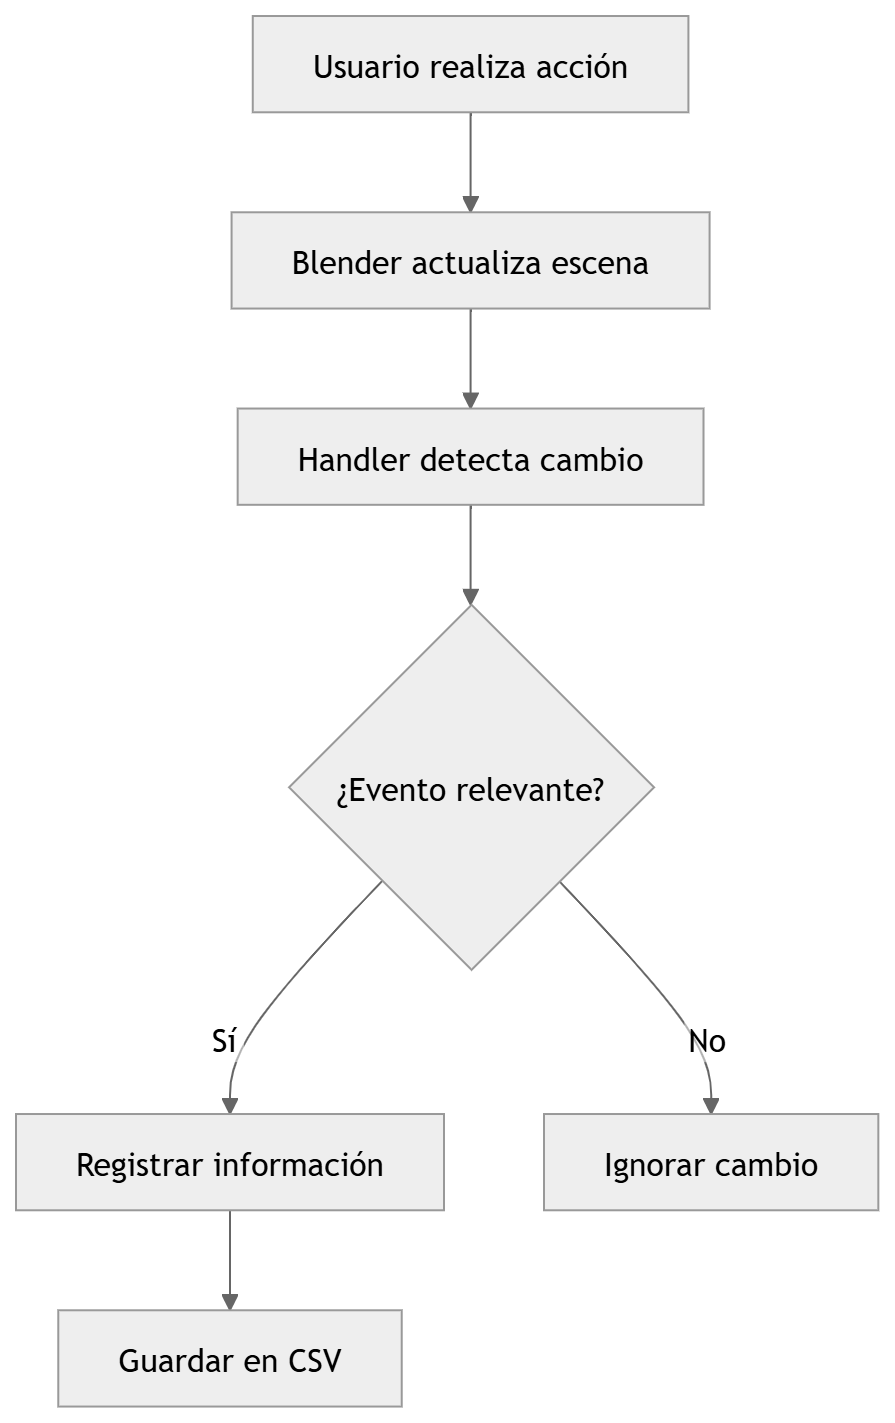
\includegraphics[width=0.5\textwidth]{diagramas/3.3flujo_eventos.png}
    \caption{Proceso general de detección y registro de eventos en Blender.}
    \label{fig:flujo_eventos}
\end{figure}

\section{Registro de eventos}

\section{Formato CSV}

Los datos que recopila el sistema se almacenan en archivos con formato CSV.

Este formato es conveniente dividir los datos entre filas y columnas, lo que simplifica el trabajar con esa información, además de ser un formato más accesible tanto desde Blender como a través de otras herramientas externas.

En esta tarea, los archivos CSV albergan datos diversos vinculados con el trabajo de modelado, como el tiempo transcurrido, la ubicación de los objetos, sus transformaciones o ciertos ajustes efectuados en el modelo durante el curso del trabajo del usuario.

La Figura~\ref{fig:csv_example} muestra un ejemplo de los datos generados por el addon de captura.

% 3.4 Formato CSV
\begin{figure}[H]
    \centering
    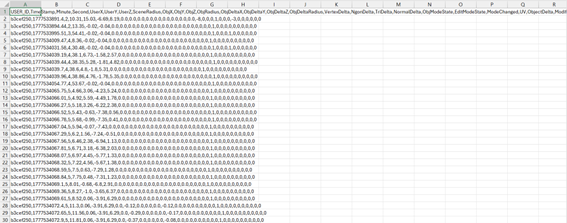
\includegraphics[width=0.9\textwidth]{diagramas/csv_example.png}
    \caption{Ejemplo de archivo CSV generado automáticamente durante una sesión de modelado.}
    \label{fig:csv_example}
\end{figure}

\section{Tipos de datos recopilados}

El sistema guarda diferentes tipos de datos para entender cómo va cambiando el modelo y cómo el usuario trabaja en la escena.

\subsection{Datos temporales}

Son datos relacionados con el tiempo que se dedica a modelar, como:

\begin{itemize}
\item cuánto duran las sesiones,
\item las pausas,
\item el tiempo entre una acción y otra,
\item o la frecuencia con la que ocurren las cosas.
\end{itemize}

Con esta información podemos ver cómo es el ritmo de trabajo del usuario y encontrar patrones de tiempo mientras modela.

\subsection{Datos espaciales}

Tienen que ver con la posición y el movimiento de los objetos, por ejemplo:

\begin{itemize}
\item coordenadas,
\item transformaciones (rotaciones, escalas),
\item desplazamientos,
\item o cómo se mueven los objetos por la escena.
\end{itemize}

Estos datos nos ayudan a entender cómo se organizan las acciones dentro del espacio 3D.

\subsection{Datos estructurales}

Están relacionados con la geometría del modelo, cosas como:

\begin{itemize}
\item el número de vértices,
\item caras,
\item modificadores que se aplican,
\item cómo cambia la malla,
\item o cualquier otro cambio en la geometría.
\end{itemize}

Con estos datos podemos ver cómo de complejo se vuelve el modelo a medida que se va diseñando.

\section{Definición de métricas}

Las métricas son valores que calculamos usando los datos que hemos registrado. La idea es que nos ayuden a entender mejor lo que hace el usuario y cómo evoluciona el modelo.

Algunas de las métricas que usa nuestro sistema son:

\begin{itemize}
\item el tiempo total que se dedica a modelar,
\item la velocidad con la que se modifica la geometría,
\item cuántas operaciones se han hecho,
\item con qué frecuencia se cambia de modo,
\item lo compleja que es la geometría de la escena,
\item o la cantidad de vértices que se han creado o borrado.
\end{itemize}

Estas métricas sirven para convertir los datos que recogemos en información que nos ayuda mucho a analizar cómo ha sido todo el proceso de modelado.

\section{Visualización de datos y gráficos}

Cuando ya tenemos los datos guardados y procesados, el sistema puede crear diferentes gráficos y dibujos para que sea más fácil entenderlos.

Por ejemplo, podemos ver:

\begin{itemize}
\item gráficas que muestran el tiempo,
\item gráficos que representan los cambios entre las distintas metricas,
\item gráficos que enseñan cómo ha cambiado la geometría,
\item y también podemos ver visualizaciones en 3D directamente dentro de Blender.
\end{itemize}

Esta figura muestra una representación de cuatro criterios relevantes para identificar patrones en la forma de operar del usuario y facilitar una comprensión más profunda de la evolución del proceso de modelado al transcurrir el tiempo.

Figura \ref{fig:radar_plot} ilustra una gráfica radar creada basándose en cuatro parámetros distintos.

\begin{figure}[H]
\centering
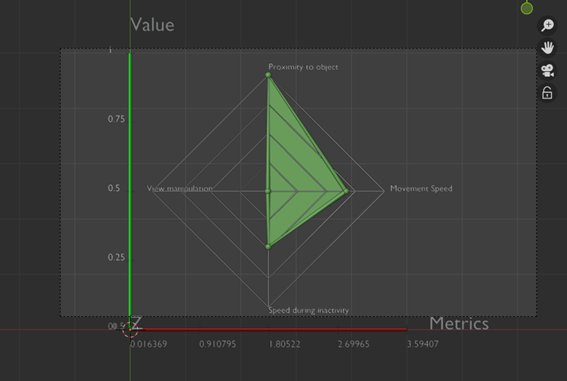
\includegraphics[
    width=\textwidth,
    height=0.7\textheight,
    keepaspectratio
]{diagramas/radar.png}
\caption{Ejemplo de visualización de datos dentro del sistema.}
\label{fig:radar_plot}
\end{figure}



